\section{Layer PerCom}
\label{layer_percom_section}

The following considerations are based on the design pattern extensions introduced
in section \ref{design_principles_section}. The terms \emph{Mapper} and \emph{Assembler}
are converted and merged into the term \emph{Translator}.

\begin{figure}[ht]
    \begin{center}
       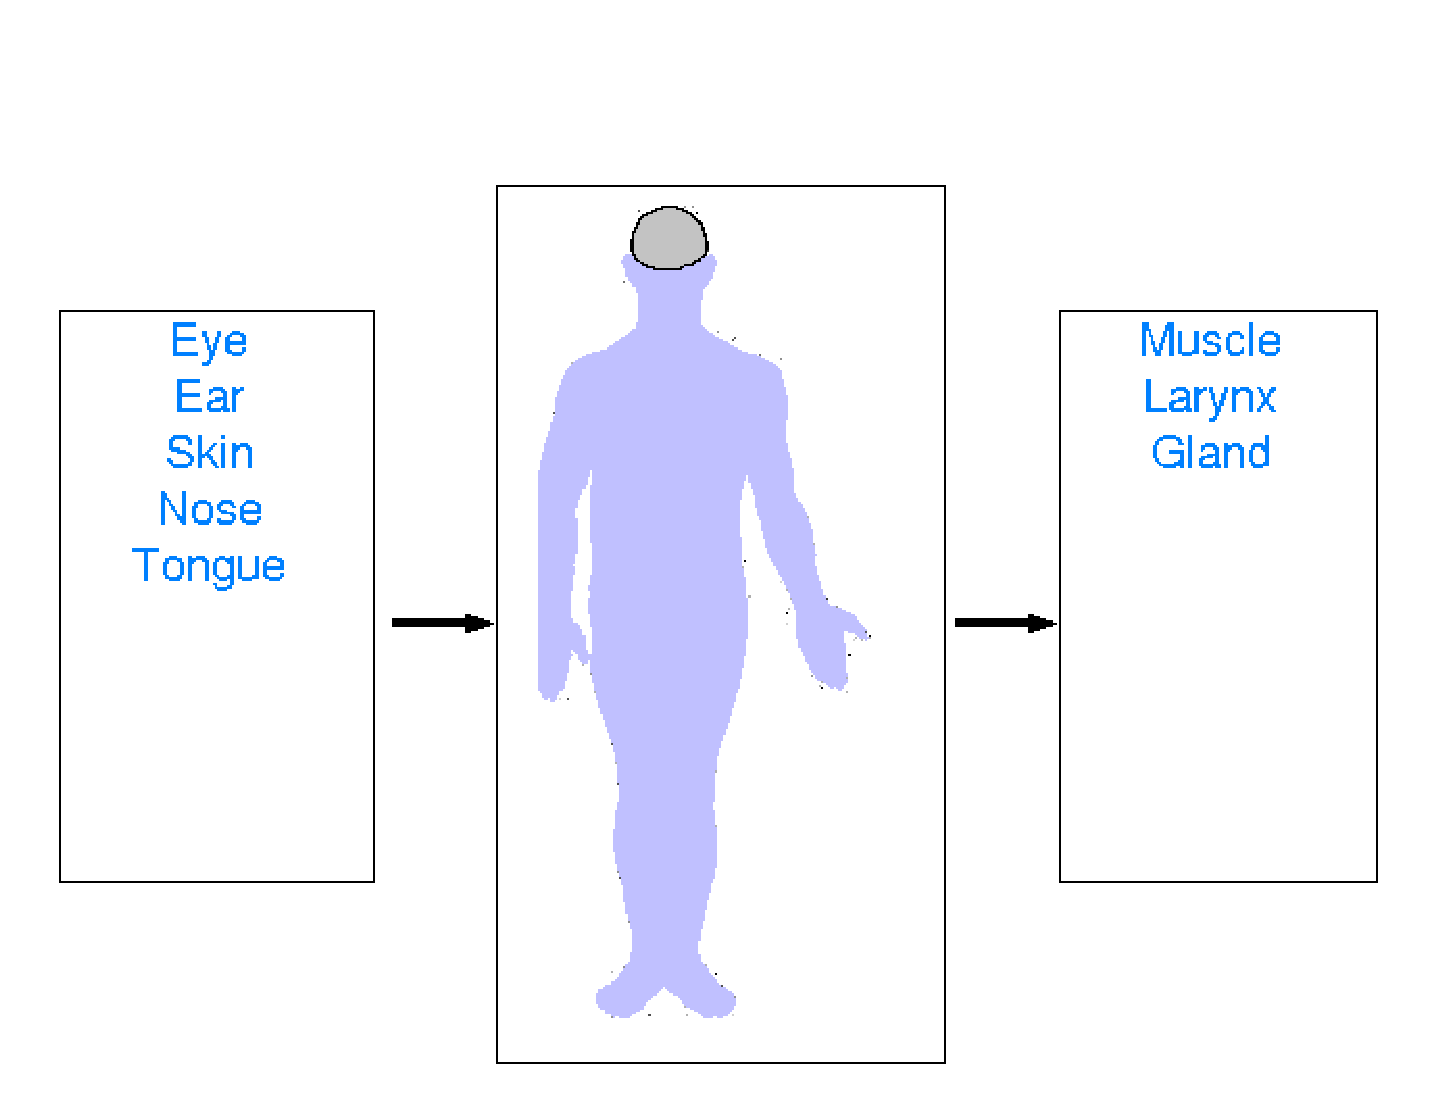
\includegraphics[scale=0.3]{images/human_being_as_system.eps}
       \caption{Human Being as System (Body) with Model (Brain)}
       \label{human_being_as_system_figure}
    \end{center}
\end{figure}

Following the CYBOP approach, nature - in our case the Human body - will be
considered next. Humans have organs responsible for information input and output
(figure \ref{human_being_as_system_figure}). In between input and output, the
information is processed by the brain that contains a specific abstract model
of the surrounding real world. The human brain consists of several regions, each
being responsible for a special task, such as the optical region for seeing or the
cerebral cortex for actual information processing which possibly leads to awareness.

\begin{figure}[ht]
    \begin{center}
       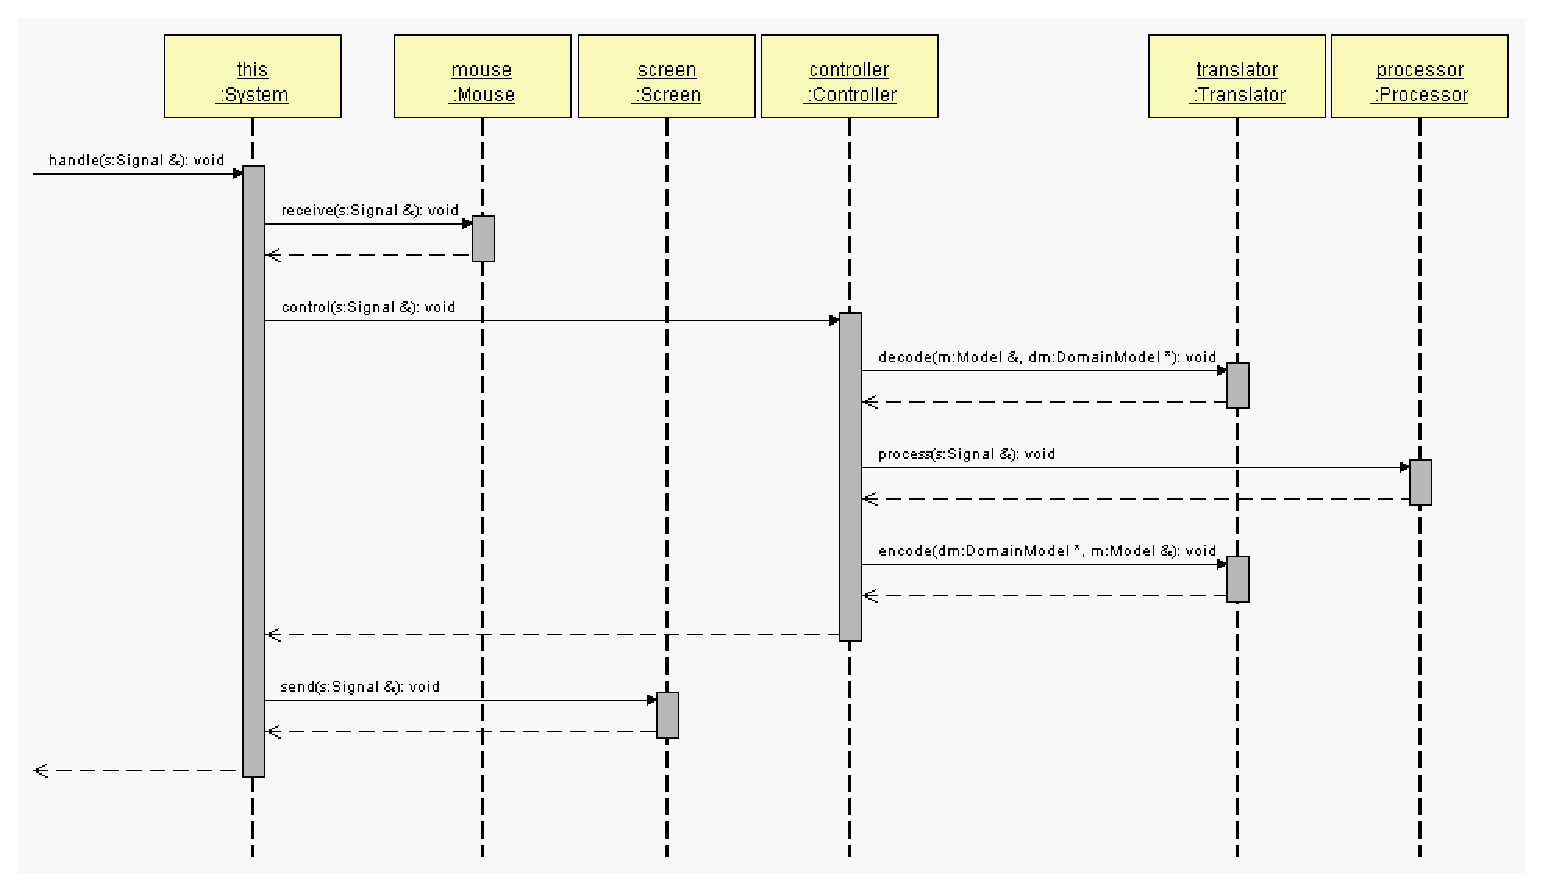
\includegraphics[scale=0.32]{images/sequence_diagram.eps}
       \caption{Signal Processing as UML Sequence Diagram}
       \label{sequence_diagram_figure}
    \end{center}
\end{figure}

The following example is to demonstrate a typical information processing procedure
(figure \ref{sequence_diagram_figure}):
One human \emph{System} wants to send another human \emph{System} a message.
It decides for an acoustical \emph{Signal}, formulates a sentence and talks to
the other human \emph{System} (\emph{handle} method). The other human receives the
\emph{Signal} across its ear organ (\emph{Keyboard}, \emph{Mouse}, \emph{Network}).
The \emph{Signal} is then forwarded to the receiver's brain (\emph{Controller})
where a special \emph{Region} responsible for acoustics (\emph{Translator})
translates the data (\emph{decode} method) contained in the \emph{Signal} and sorts
them into the human's abstract model of the surrounding real world (\emph{DomainModel}).
Processing of the signal happens in the cerebral cortex of the brain (\emph{Processor}).
If the addressed listener wants to send an answer \emph{Signal}, it may do so by
triggering a muscle reaction. For this to happen, the motoric brain region (\emph{Translator})
needs to translate (\emph{encode} method) abstract model (\emph{DomainModel}) data
into a special communication model for the answer signal. Finally, the answer
signal will be sent as muscle action (data display on \emph{Screen}).\\
As can be seen, there is always a translator that is able to map domain model data
to communication model data (\emph{encode} method) and back (\emph{decode} method).
Depending on which communication medium is used, different translators need to be
applied (figure \ref{translator_classes_figure}).

\begin{figure}[ht]
    \begin{center}
       \includegraphics[scale=0.24]{images/class_diagram.eps}
       \caption{Translator Classes in a UML Class Diagram}
       \label{translator_classes_figure}
    \end{center}
\end{figure}

Every system has exactly one domain model but communication models of arbitrary
type can be added anytime (figure \ref{translators_figure}). Every translator knows
only how to translate between the domain model and a special communication model.
Direct translation between communication models is forbidden as it would break the
flexibility of the whole framework. In other words, translations always have to be
done via the domain model.

\begin{figure}[ht]
    \begin{center}
       \includegraphics[scale=0.4]{images/layer_percom.eps}
       \caption{Translators accessing various Models}
       \label{translators_figure}
    \end{center}
\end{figure}

This highly flexible and extensible architecture is absolutely transparent to
the user. S/He will not know whether the current communication is with the local
file system, a database or a remote process on another machine. However, this
transparency causes a number of problems. Surely, the most common question is
how to ensure consistence, security and minimum redundance? The following two
sections give an answer to the first part of this question -- consistence and
uniqueness of data sets. Maximizing security and minimizing redundancy have to
be analysed in future works.

\subsection{Object ID (OID)}
\label{object_id_section}

Most database systems provide an own algorithm to generate primary keys for the
tables. But the applications that use the \emph{Layer PerCom} architecture shall
also be able to work if a database server is not reachable, e.g. due to a network
failure. Thats why the keys are generated locally, by each application.
Based on the assumption that every host in a network has a network card, it thereby
has a unique internet address. This number is concatinated with an exact time stamp
(nanoseconds). That is why the OID is unique in the global network and unique in time.\\
The proposed approach uses the OID as file name for local storage and the same
OID as primary key in the main table of the database. Therewith, both models can
be mapped to each other. Of course, it is necessary to avoid overwriting of new
data in the database. If, for example, a network connection is cut and a little
later, one wants to get data from the local files and write them up in the restored
central database, it has to be made sure that nobody else has modified the data
during the offline-time. That is why there is another technique to ensure this
-- the time stamp.

\subsection{Time stamp}
\label{time_stamp_section}

Most database developers will know this technique. Each table has a separate
column for storing the time at which the data were written into this table.
If someone requests information from the database, the time stamp is delivered
as well. After modifying the data, they have to be written back into the database.
At this time, both timestamps (the one in the database table and the one delivered
before) are compared. If there is a difference, the data were modified by another
user. Then, one has to care about the update without overwriting the new data in
the table.
